\documentclass[12pt]{article}

% For arXiv submission - single column format
\usepackage[letterpaper, margin=1in]{geometry}
\usepackage{times}  % Use Times font for better readability
\usepackage{amsmath}
\usepackage{amssymb}
\usepackage{amsthm}
\usepackage{listings}
\usepackage{algorithm}
\usepackage{algpseudocode}  % This replaces algorithmic
\usepackage{stmaryrd}  % For semantic brackets
\usepackage{tikz}
\usepackage{pgfplots}
\usepackage{graphicx}
\usepackage{subcaption}
\usepackage{booktabs}
\usepackage{xcolor}
\usepackage{url}
\usepackage{hyperref}

% Define colors for syntax highlighting
\definecolor{aperture}{RGB}{139, 69, 19}
\definecolor{keyword}{RGB}{0, 0, 255}
\definecolor{comment}{RGB}{0, 128, 0}
\definecolor{string}{RGB}{255, 0, 0}

% Configure listings for Lisp
\lstdefinestyle{lisp}{
    basicstyle=\footnotesize\ttfamily,
    keywordstyle=\color{keyword}\bfseries,
    commentstyle=\color{comment}\itshape,
    stringstyle=\color{string},
    showstringspaces=false,
    breaklines=true,
    frame=single,
    numbers=left,
    numberstyle=\tiny\color{gray},
    emph={?},
    emphstyle=\color{aperture}\bfseries,
}

\lstset{style=lisp}

% Theorems and definitions
\newtheorem{theorem}{Theorem}
\newtheorem{lemma}[theorem]{Lemma}
\newtheorem{corollary}[theorem]{Corollary}
\newtheorem{definition}[theorem]{Definition}
\newtheorem{property}[theorem]{Property}
\newtheorem{example}[theorem]{Example}
\newtheorem{remark}[theorem]{Remark}

\begin{document}

\title{\Large \bf Apertures: Linguistic Abstractions for\\Controlled Information Disclosure in Distributed Computation}

\author{
Alexander Towell\\
Department of Computer Science\\
Southern Illinois University Edwardsville\\
\texttt{atowell@siue.edu}
}

\date{\today}

\maketitle

\begin{abstract}
We introduce \textit{apertures}, a novel programming language construct that enables controlled information disclosure in distributed computation through structural separation of sensitive and non-sensitive program components. Unlike cryptographic approaches such as homomorphic encryption or secure multi-party computation protocols, apertures provide a linguistic abstraction where holes in expressions serve as placeholders for private values. While apertures can be partially evaluated and optimized by untrusted parties, we explicitly acknowledge that the combination of program structure and computed results may leak information about aperture values through algebraic reasoning. We formalize these leakage bounds and show how integration with oblivious functions can mitigate—though not eliminate—such leakage. 

We present a formal semantics for aperture-based computation with explicit leakage quantification, prove properties including semantic preservation under partial evaluation, and demonstrate how apertures enable novel computational patterns including multi-party progressive refinement. Our prototype implementation in C++23 shows that apertures can achieve practical performance as a coordination mechanism for distributed computation. We provide microbenchmarks comparing aperture operations against baseline implementations, though we acknowledge that comprehensive real-world evaluation remains future work. Our preliminary results suggest apertures may offer a useful tradeoff between computational efficiency and information disclosure control, particularly when combined with oblivious encoding techniques.

The key insight is that by controlling evaluation depth through strategic aperture placement, we can maximize computation on untrusted infrastructure while maintaining precise control over information disclosure. We further show how apertures naturally support symbolic reasoning, enabling hybrid symbolic-neural computation where language models can provide contextual hole-filling during evaluation.
\end{abstract}

\vspace{1em}
\noindent\textbf{Keywords:} privacy-preserving computation, partial evaluation, programming languages, distributed systems, secure multi-party computation, information flow control

\vspace{1em}
\noindent\textbf{arXiv categories:} cs.CR (Cryptography and Security), cs.PL (Programming Languages), cs.DC (Distributed Computing)

\section{Introduction}

The proliferation of cloud computing and distributed systems has created an fundamental tension in modern software architecture: the desire to leverage powerful remote computational resources conflicts with the need to protect sensitive data. Current solutions to this dilemma fall broadly into two categories, each with significant limitations.

Cryptographic approaches, exemplified by Fully Homomorphic Encryption (FHE)~\cite{gentry2009fully} and Secure Multi-Party Computation (MPC)~\cite{yao1982protocols}, provide strong theoretical guarantees but suffer from computational overheads often exceeding 1000× for realistic workloads. Hardware-based solutions using trusted execution environments~\cite{costan2016intel} require specialized infrastructure and trust in hardware vendors. Meanwhile, purely policy-based approaches rely on legal frameworks and auditing, providing no technical enforcement of privacy guarantees.

We propose a different approach: \textit{apertures}, a linguistic abstraction for managing information disclosure in distributed computation through structural program transformation. An aperture, denoted \texttt{?variable}, represents a hole in an expression—a placeholder for a value that is unknown during partial evaluation. While this enables untrusted parties to optimize and transform programs, we must be clear: apertures do not provide cryptographic privacy. The combination of program structure and results can leak information. This paper explores the tradeoffs, quantifies the leakage, and shows when apertures provide a useful coordination mechanism despite their limitations.

\subsection{Motivating Example}

Consider a medical research scenario where multiple hospitals want to jointly train a machine learning model without sharing patient data. Using apertures, we can express this as:

\begin{lstlisting}
(define (federated-gradient data)
  (let ((model-params (initialize-model))
        (batch-size 100))
    (map (lambda (hospital-data)
           (let ((gradient 
                  (compute-local-gradient 
                    model-params 
                    ?{hospital-data})))
             (scale gradient (/ 1 batch-size))))
         data)))
\end{lstlisting}

The crucial insight is that \texttt{?hospital-data} acts as an aperture—the expression can be partially evaluated to optimize the gradient computation structure, determine the scaling factor, and prepare the aggregation, all without accessing the actual patient data. Each hospital fills its aperture locally, computes its gradient contribution, and shares only the aggregate statistics.

\subsection{Contributions}

This paper makes the following contributions:

\begin{enumerate}
    \item \textbf{Aperture Calculus}: We formalize apertures as a core language construct with precise operational semantics, including rules for partial evaluation that preserve semantic equivalence while maintaining privacy.
    
    \item \textbf{Computation Depth Analysis}: We demonstrate how strategic aperture placement enables deep computation trees to be evaluated on untrusted infrastructure, with apertures acting as evaluation barriers only at necessary privacy boundaries.
    
    \item \textbf{Multi-Party Progressive Refinement}: We introduce a novel computational pattern where multiple parties can progressively refine a computation in rounds, with each party filling specific apertures to enable further evaluation by subsequent parties.
    
    \item \textbf{Symbolic Inference Integration}: We show how apertures naturally support symbolic reasoning and can be dynamically filled through language model inference, enabling hybrid symbolic-neural computation.
    
    \item \textbf{Implementation and Evaluation}: We provide a complete implementation in a Lisp-like language and demonstrate practical performance across diverse application domains.
\end{enumerate}

\section{Background and Related Work}

\subsection{Partial Evaluation}

Partial evaluation~\cite{jones1993partial} is a program transformation technique that specializes programs with respect to known inputs. Traditional partial evaluation assumes complete knowledge of which inputs are static (known at specialization time) versus dynamic (known only at runtime). The Futamura projections demonstrate how partial evaluators can generate compilers and compiler generators.

Apertures differ from traditional partial evaluation in three fundamental ways:
\begin{enumerate}
    \item \textbf{Three-valued binding times}: Beyond static/dynamic, apertures introduce \textit{opaque} values that halt evaluation but preserve structure. This enables distributed evaluation without information disclosure.
    
    \item \textbf{Resumable evaluation}: Traditional partial evaluation produces residual programs. Apertures produce pausable computations that can be resumed when values become available, enabling multi-party protocols.
    
    \item \textbf{Information hiding vs. specialization}: Partial evaluation aims to optimize by specializing code. Apertures aim to hide information while enabling computation, accepting performance overhead for privacy.
\end{enumerate}

The relationship with binding-time analysis~\cite{nielson1992two} is particularly relevant. While BTA determines when values become available for optimization, apertures mark which values must remain hidden for privacy. This can be viewed as an \textit{inverse binding-time analysis} where we identify values that must NOT be bound during distributed evaluation.

Online partial evaluation, which interleaves specialization with execution, shares our goal of incremental computation. However, online specializers make binding-time decisions dynamically for performance, while apertures enforce static privacy boundaries regardless of runtime information availability.

\subsection{Information Flow Control}

Language-based information flow control~\cite{sabelfeld2003language} tracks how information propagates through programs. Security type systems~\cite{volpano1996sound} statically verify non-interference properties. Apertures provide a complementary approach: rather than tracking information flow, they structurally prevent it through evaluation barriers.

Dynamic information flow systems~\cite{austin2009efficient} monitor data propagation at runtime. Our approach differs fundamentally—apertures are not tags or labels but first-class language constructs that actively shape evaluation.

\subsection{Secure Computation}

Fully homomorphic encryption~\cite{gentry2009fully} enables computation on encrypted data but with severe performance penalties. Recent optimizations~\cite{cheon2017homomorphic} have improved performance but still incur overheads of 100-10,000× for typical operations.

Secure multi-party computation~\cite{goldreich1987play} enables joint computation over private inputs through cryptographic protocols. Apertures offer a different tradeoff: weaker cryptographic guarantees but dramatically better performance and simpler programming models.

\subsection{Symbolic Execution}

Symbolic execution~\cite{king1976symbolic} analyzes programs by treating inputs as symbolic values. Apertures can be viewed as a form of controlled symbolic execution where certain symbols (apertures) are never concretized during distributed evaluation. This connection enables integration with SMT solvers for constraint propagation and verification.

\section{The Aperture Calculus}

\subsection{Syntax and Core Semantics}

We formalize apertures within a lambda calculus extended with holes. Let $\mathcal{V}$ be a set of values, $\mathcal{X}$ a set of variables, and $\mathcal{H}$ a set of hole identifiers.

\begin{definition}[Aperture Calculus Syntax]
\begin{align}
e ::= \quad & v \quad \text{(values)} \\
    | \quad & x \quad \text{(variables)} \\
    | \quad & ?h \quad \text{(apertures)} \\
    | \quad & \lambda x.e \quad \text{(abstraction)} \\
    | \quad & e_1 \, e_2 \quad \text{(application)} \\
    | \quad & \text{let } x = e_1 \text{ in } e_2 \quad \text{(let-binding)} \\
    | \quad & \text{op}(e_1, ..., e_n) \quad \text{(operations)}
\end{align}
\end{definition}

The evaluation relation $\rightarrow$ is defined by standard beta-reduction extended with aperture-aware rules:

\begin{align}
(\lambda x.e) \, v &\rightarrow e[x \mapsto v] \\
\text{let } x = v \text{ in } e &\rightarrow e[x \mapsto v] \\
\text{op}(v_1, ..., v_n) &\rightarrow \delta(\text{op}, v_1, ..., v_n) \\
\text{op}(..., ?h, ...) &\rightarrow \text{op}(..., ?h, ...) \quad \text{(aperture barrier)}
\end{align}

The critical rule is the aperture barrier: operations containing apertures cannot be reduced further, preserving the structural form for later filling.

\subsection{Partial Evaluation Semantics}

We define partial evaluation as evaluation in an incomplete environment:

\begin{definition}[Partial Evaluation]
Given expression $e$ and partial environment $\rho : \mathcal{X} \rightharpoonup \mathcal{V}$, partial evaluation $\llbracket e \rrbracket_\rho$ produces a residual expression:

\begin{align}
\llbracket v \rrbracket_\rho &= v \\
\llbracket x \rrbracket_\rho &= \begin{cases}
    \rho(x) & \text{if } x \in \text{dom}(\rho) \\
    x & \text{otherwise}
\end{cases} \\
\llbracket ?h \rrbracket_\rho &= ?h \\
\llbracket e_1 \, e_2 \rrbracket_\rho &= \begin{cases}
    \llbracket e'[x \mapsto v_2] \rrbracket_\rho & \text{if } \llbracket e_1 \rrbracket_\rho = \lambda x.e' \land \llbracket e_2 \rrbracket_\rho = v_2 \\
    \llbracket e_1 \rrbracket_\rho \, \llbracket e_2 \rrbracket_\rho & \text{otherwise}
\end{cases}
\end{align}
\end{definition}

\subsection{Pausable and Resumable Evaluation}

A critical architectural decision enabling apertures is our stack-based evaluation model, which naturally supports pausing evaluation at aperture boundaries and resuming when values become available. This capability, inspired by continuation-based interpreters~\cite{reynolds1972definitional,friedman1976control}, is fundamental to the aperture abstraction.

\begin{definition}[Evaluation Context]
An evaluation context $\mathcal{E}$ is a pair $(\kappa, \sigma)$ where:
\begin{itemize}
    \item $\kappa$ is a continuation stack representing pending computation
    \item $\sigma$ is an environment mapping variables to values
\end{itemize}
\end{definition}

When evaluation encounters an aperture, it captures the current context:

\begin{lstlisting}
(define (pausable-eval expr context)
  (match expr
    [?h (suspend context expr)]
    [(op e1 ... ?h ... en)
     (let ((evaluated (map-pausable eval [e1 ... ?h-1])))
       (suspend (extend-context context op evaluated) 
                ?h))]
    [_ (continue-eval expr context)]))
\end{lstlisting}

\begin{property}[Evaluation Resumability]
For any expression $e$ with evaluation paused at aperture $?h$:
$$\text{resume}(\text{pause}(e, ?h), v) = e[?h \mapsto v]$$
\end{property}

This property ensures that evaluation can be arbitrarily interleaved across trust boundaries. A server can evaluate until reaching an aperture, serialize the continuation, and return it to the client. The client fills the aperture and either continues evaluation locally or sends it back for further server processing.

\begin{example}[Continuation Passing]
Consider evaluating $(* \; (+ \; ?x \; 3) \; (- \; 10 \; ?y))$:

\begin{enumerate}
    \item Server evaluates: Pauses at $?x$, returns $\langle \lambda v.(* \; (+ \; v \; 3) \; (- \; 10 \; ?y)), \sigma \rangle$
    \item Client fills $?x = 7$: Computes $(+ \; 7 \; 3) = 10$
    \item Client sends: $(* \; 10 \; (- \; 10 \; ?y))$ back to server
    \item Server evaluates: Pauses at $?y$, returns $\langle \lambda v.(* \; 10 \; (- \; 10 \; v)), \sigma \rangle$
    \item Client fills $?y = 4$: Computes final result $60$
\end{enumerate}
\end{example}

The stack-based architecture provides several key benefits:

\textbf{Incremental Progress:} Each evaluation step before an aperture is preserved, avoiding redundant recomputation.

\textbf{Composable Contexts:} Multiple partial evaluations can be composed by merging their continuation stacks.

\textbf{Serializable State:} The evaluation context can be serialized and transmitted between parties, enabling true distributed evaluation.

\textbf{Backtracking Support:} The stack structure naturally supports speculative evaluation with rollback if constraints are violated.

\subsection{Security Properties}

We establish three fundamental security properties:

\begin{property}[Non-Interference]
Let $e$ be an expression with aperture $?h$. For any two values $v_1, v_2$, the partial evaluations are structurally equivalent:
$$\llbracket e[?h \mapsto v_1] \rrbracket_\rho \equiv_\alpha \llbracket e[?h \mapsto v_2] \rrbracket_\rho$$
where evaluation stops at aperture boundaries.
\end{property}

\begin{property}[Semantic Preservation]
Partial evaluation preserves semantics under hole filling:
$$\llbracket \llbracket e \rrbracket_{\rho_1}[?h \mapsto v] \rrbracket_{\rho_2} = \llbracket e[?h \mapsto v] \rrbracket_{\rho_1 \cup \rho_2}$$
\end{property}

\begin{property}[Computation Monotonicity]
Partial evaluation never loses computational progress:
$$\text{depth}(\llbracket e \rrbracket_\rho) \leq \text{depth}(e)$$
where depth measures the evaluation steps completed.
\end{property}

\section{Maximizing Computation Depth}

A key insight for practical aperture use is that computation can proceed deeply as long as apertures appear high in the expression tree. We formalize this through the concept of \textit{aperture depth}.

\subsection{Aperture Depth Analysis}

\begin{definition}[Aperture Depth]
The aperture depth $d_?(e)$ of expression $e$ is the minimum depth at which an aperture appears:
\begin{align}
d_?(\text{value}) &= \infty \\
d_?(?h) &= 0 \\
d_?(e_1 \, e_2) &= 1 + \min(d_?(e_1), d_?(e_2)) \\
d_?(\text{op}(e_1, ..., e_n)) &= 1 + \min_{i} d_?(e_i)
\end{align}
\end{definition}

\begin{theorem}[Computation Depth Theorem]
An expression $e$ can be evaluated to depth $d$ on an untrusted server if and only if $d < d_?(e)$.
\end{theorem}

\begin{proof}
By structural induction on the evaluation derivation. The aperture barrier rule prevents evaluation from proceeding past depth $d_?(e)$.
\end{proof}

\subsection{Strategic Aperture Placement}

Consider a complex analytical query over sensitive data:

\begin{lstlisting}
(define (analyze-transactions user-id)
  (let ((all-transactions (load-transactions user-id))
        (fraud-model (load-model "fraud-v3"))
        (risk-threshold 0.85))
    (filter (lambda (tx)
              (> (apply-model fraud-model 
                            (extract-features tx))
                 risk-threshold))
            ?{all-transactions})))
\end{lstlisting}

By placing the aperture at \texttt{?all-transactions}, we enable the untrusted server to:
\begin{itemize}
    \item Load and prepare the fraud detection model (potentially expensive)
    \item Set up the filtering predicate
    \item Optimize the feature extraction pipeline
    \item Pre-compile the model application
\end{itemize}

Only the actual transaction data remains private. The server performs substantial computation, preparing an optimized execution plan that the client simply fills and runs.

\subsection{Depth-Optimal Transformation}

We can automatically transform programs to maximize computation depth:

\begin{algorithm}
\caption{Aperture Lifting Transformation}
\begin{algorithmic}[1]
\Require Expression $e$, Privacy set $P$
\Ensure Transformed expression $e'$ with maximum $d_?(e')$
\Procedure{LiftApertures}{$e, P$}
    \If{$e \in P$}
        \State \Return $?\text{fresh()}$
    \ElsIf{$e = \text{op}(e_1, ..., e_n)$}
        \State $lifted \gets \text{map}(\lambda e_i. \text{LiftApertures}(e_i, P), [e_1, ..., e_n])$
        \If{$\text{any}(\text{isAperture}, lifted)$}
            \State \textbf{return} $\text{op}(lifted)$
        \Else
            \State \textbf{return} $e$ \Comment{Keep computation together}
        \EndIf
    \Else
        \State \textbf{return} $e$
    \EndIf
\EndProcedure
\end{algorithmic}
\end{algorithm}

\section{Information Leakage and Trust Domains}

\subsection{The Fundamental Leakage Problem}

\textbf{We must be clear from the outset: apertures leak information.} This is not an implementation flaw but a fundamental property of the approach. When an untrusted server sees both the program structure and computed results, it can often deduce aperture values through algebraic reasoning. This section quantifies this leakage and discusses when it might be acceptable.

\begin{example}[Simple Leakage]
Consider the expression $(+ \; ?x \; 10)$:
\begin{enumerate}
    \item Untrusted server pauses at $?x$, sends to trusted party
    \item Trusted party fills $?x = 4$, evaluates to $14$
    \item Untrusted server receives $14$, infers $?x = 4$
\end{enumerate}
\end{example}

This leakage is not a bug but a fundamental property: if the untrusted party sees both the expression structure and the final result, it can often deduce aperture values through algebraic reasoning.

\subsection{Quantifying Information Leakage}

We formalize information leakage through the lens of information theory:

\begin{definition}[Aperture Entropy]
For aperture $?h$ with domain $\mathcal{D}_h$ and expression $e$, the entropy is:
$$H(?h | e) = -\sum_{v \in \mathcal{D}_h} P(v) \log P(v)$$
\end{definition}

\begin{definition}[Leakage Function]
The information leaked when evaluating $e$ with aperture $?h$ is:
$$L(e, ?h) = H(?h) - H(?h | \text{observe}(e[?h]))$$
\end{definition}

\begin{property}[Leakage Bounds]
For expression $e$ with aperture $?h$:
\begin{itemize}
    \item If $e = ?h$, then $L(e, ?h) = H(?h)$ (complete leakage)
    \item If $e = f(?h)$ where $f$ is injective, then $L(e, ?h) = H(?h)$
    \item If $e = f(?h)$ where $f$ is constant, then $L(e, ?h) = 0$
    \item If $e = f(?h_1, ..., ?h_n)$ with $n > 1$, then $L(e, ?h_i) \leq H(?h_i)$
\end{itemize}
\end{property}

\subsection{Trust Domain Architecture}

To manage information leakage, we introduce \textit{trust domains} with explicit routing rules:

\begin{definition}[Trust Domain]
A trust domain $\mathcal{T}$ is a tuple $(P, A, R, S)$ where:
\begin{itemize}
    \item $P$ is a set of parties
    \item $A \subseteq \mathcal{H}$ is the set of apertures this domain can fill
    \item $R : \mathcal{H} \rightarrow \mathcal{T}$ is a routing function
    \item $S : \mathcal{P}(P) \rightarrow \{0,1\}$ indicates allowed information sharing
\end{itemize}
\end{definition}

\begin{lstlisting}
(define-trust-domain medical-data
  :parties #{hospital-a hospital-b}
  :fills ?{patient-*}
  :route-to medical-processor
  :no-share-with #{insurance-companies})

(define-trust-domain financial-data
  :parties #{bank-1 bank-2}
  :fills ?{account-* transaction-*}
  :route-to financial-processor
  :no-share-with #{medical-data})
\end{lstlisting}

\subsection{Algebraic Obfuscation}

When aperture values cannot be hidden, we can increase the algebraic complexity to prevent inference:

\begin{theorem}[Inference Hardness]
For expression $e = f(?h_1, ..., ?h_n)$ where $f$ is a polynomial of degree $d$, determining aperture values from the result requires solving a system with:
\begin{itemize}
    \item Variables: $n$
    \item Constraints: 1 (the observed output)
    \item Degrees of freedom: $n - 1$
\end{itemize}
When $n > 1$ and $d > 1$, the problem becomes computationally hard for large domains.
\end{theorem}

\begin{example}[Complex Expression Protection]
Consider $z = ?x \cdot 2 - \sqrt{?y}$:
\begin{itemize}
    \item Given $z = 10$: infinite solutions $(x,y)$ exist
    \item E.g., $(x=7, y=16)$, $(x=8, y=36)$, $(x=9, y=64)$
    \item Without additional constraints, aperture values remain hidden
\end{itemize}
\end{example}

\subsection{Mitigation Strategies}

We propose several strategies to mitigate information leakage:

\subsubsection{Onion Routing of Computations}

Inspired by Tor, we route computations through multiple untrusted parties:

\begin{lstlisting}
(define (onion-eval expr apertures)
  (let* ((servers (shuffle untrusted-servers))
         (layers (partition apertures (length servers))))
    (fold (lambda (server layer-apertures partial)
            (server-eval server partial layer-apertures))
          expr
          servers
          layers)))
\end{lstlisting}

Each server sees only a fragment of the computation, making reconstruction difficult without collusion.

\subsubsection{Differential Privacy Noise}

Add calibrated noise to aperture values before evaluation:

\begin{lstlisting}
(define (dp-fill aperture value epsilon)
  (let ((sensitivity (compute-sensitivity aperture))
        (noise (laplace 0 (/ sensitivity epsilon))))
    (+ value noise)))
\end{lstlisting}

This provides statistical privacy guarantees even when values are observed.

\subsubsection{Homomorphic Aperture Filling}

For critical apertures, use homomorphic encryption for the filling step:

\begin{lstlisting}
(define (secure-fill aperture value)
  (if (critical? aperture)
      (fhe-encrypt value)
      value))
\end{lstlisting}

This combines the efficiency of apertures with cryptographic protection where needed.

\subsubsection{Aperture Bundling}

Group related apertures to prevent individual inference:

\begin{lstlisting}
(define (bundle-apertures expr)
  (let ((related (find-related-apertures expr)))
    (replace-with-composite 
      expr 
      related 
      (make-bundle-aperture related))))
\end{lstlisting}

The trusted party fills all bundled apertures simultaneously, returning only the aggregate result.

\section{Multi-Party Progressive Refinement}

Building on trust domains, apertures enable a novel computational pattern where multiple parties progressively refine a computation through rounds of aperture filling, with careful management of information flow.

\subsection{Round-Robin Evaluation Protocol}

Consider three parties computing a joint function where each party's input depends on partial results from others:

\begin{lstlisting}
(define (three-party-auction)
  (let ((base-price 1000))
    (let ((alice-bid (+ base-price 
                       (* ?{alice-value} 
                          (market-adjustment))))
          (bob-bid (+ base-price 
                     (* ?{bob-value} 
                        (if (> alice-bid 1500) 
                            0.9 1.1))))
          (carol-bid (+ base-price
                       (* ?{carol-value}
                          (average alice-bid bob-bid)))))
      (list alice-bid bob-bid carol-bid))))
\end{lstlisting}

The evaluation proceeds in rounds:

\textbf{Round 1:} Public server partially evaluates, computing \texttt{market-adjustment()} and preparing structure.

\textbf{Round 2:} Alice fills \texttt{?alice-value}, enables evaluation of her bid and the condition for Bob's adjustment factor.

\textbf{Round 3:} Bob fills \texttt{?bob-value}, enabling computation of his bid and the average for Carol.

\textbf{Round 4:} Carol fills \texttt{?carol-value} and completes evaluation.

Each party sees only the information necessary for their decision, and the computation proceeds without revealing individual valuations.

\subsection{Formal Protocol}

We formalize the multi-party protocol as a state machine:

\begin{definition}[Progressive Refinement Protocol]
A protocol state is a tuple $(e, \sigma, \pi)$ where:
\begin{itemize}
    \item $e$ is the current residual expression
    \item $\sigma : \mathcal{H} \rightarrow \mathcal{V}$ is the accumulated substitution
    \item $\pi : \mathbb{N} \rightarrow \mathcal{P}(\mathcal{H})$ maps rounds to fillable apertures
\end{itemize}

The protocol transition for party $p$ in round $i$:
$$(e, \sigma, \pi) \xrightarrow{p, \phi_p} (e', \sigma', \pi)$$
where $\phi_p : \pi(i) \cap \text{owned}(p) \rightarrow \mathcal{V}$ is $p$'s filling function.
\end{definition}

\begin{theorem}[Protocol Completeness]
A progressive refinement protocol terminates successfully iff the dependency graph of apertures is acyclic.
\end{theorem}

\subsection{Incentive Compatibility}

The round-robin structure creates natural incentives for participation:

\begin{property}[Monotonic Information Revelation]
In each round, the information revealed to party $p$ is exactly the minimum required for $p$ to make their contribution.
\end{property}

This property ensures that parties cannot gain advantage by delaying participation or attempting to extract more information than necessary.

\section{Oblivious Domain Computation with Apertures}

\subsection{Bridging Apertures and Oblivious Functions}

While apertures provide structural privacy through evaluation barriers, they can leak information when computations move between trust domains (as discussed in Section 5). We present a novel solution: integrate apertures with oblivious functions that operate in an encoded domain where all values appear uniformly random.

\begin{definition}[Oblivious Aperture]
An oblivious aperture combines:
\begin{itemize}
    \item An aperture $?h$ representing a private value
    \item An oblivious encoding function $\mathsf{encode}: V \rightarrow \hat{V}$
    \item An oblivious decoding function $\mathsf{decode}: \hat{V} \rightarrow V$
\end{itemize}
such that computations proceed in the oblivious domain $\hat{V}$ where all values appear uniform.
\end{definition}

\subsection{The Oblivious Evaluation Protocol}

The key insight is that trusted parties can encode results back into the oblivious domain before returning them:

\begin{lstlisting}
(define (oblivious-aperture-eval expr)
  (match expr
    [?h 
     ;; Trusted party fills aperture
     (let ((plaintext (get-aperture-value ?h))
           (encoded (encode-oblivious plaintext)))
       ;; Return encoded value, not plaintext
       (resume-with encoded))]
    [(op args...)
     ;; Operate in oblivious domain
     (oblivious-op (map oblivious-aperture-eval args))]))
\end{lstlisting}

\begin{theorem}[Information Hiding via Oblivious Encoding]
If encoding function $\mathsf{encode}$ produces uniformly distributed outputs, then for expression $e$ with aperture $?h$:
$$I(e[?h]; \mathsf{encode}(v)) = 0$$
where $v$ is the aperture's true value and $I$ denotes mutual information.
\end{theorem}

\subsection{Hash-Based Oblivious Functions}

Following the Bernoulli construction paradigm, we implement oblivious functions using hash encodings:

\begin{definition}[Oblivious Function via Hash Encoding]
For function $f: X \rightarrow Y$, construct $\hat{f}: \hat{X} \rightarrow \hat{Y}$:
\begin{enumerate}
    \item Encode inputs: $\hat{x} = h(x \| \text{seed})$
    \item Define valid encodings: $|\text{ValidEnc}(y)| \propto 1/\text{freq}(y)$
    \item Compute: $\hat{f}(\hat{x}) = h'(\hat{x}) \in \text{ValidEnc}(f(\text{decode}(\hat{x})))$
    \item Invalid inputs map to uniform random outputs
\end{enumerate}
\end{definition}

This construction ensures:
\begin{itemize}
    \item All observable values are uniformly distributed hashes
    \item Invalid inputs provide free noise, enhancing privacy
    \item Composition preserves uniformity through the computation
\end{itemize}

\subsection{Integration with Aperture Evaluation}

When an untrusted server encounters an aperture during evaluation:

\begin{algorithm}
\caption{Oblivious Aperture Protocol}
\begin{algorithmic}[1]
\State Server pauses at aperture $?h$, sends context to trusted party
\State Trusted party retrieves plaintext value $v$ for $?h$
\State Trusted party computes $\hat{v} = \mathsf{encode}(v)$ 
\State Trusted party returns oblivious value $\hat{v}$ to server
\State Server continues evaluation in oblivious domain with $\hat{v}$
\State Final result remains in oblivious domain or decoded by client
\end{algorithmic}
\end{algorithm}

\begin{example}[Oblivious Arithmetic]
Consider $(+ \; (* \; ?x \; 2) \; ?y)$ where $x=5, y=3$:
\begin{enumerate}
    \item Server pauses at $?x$, sends to trusted party A
    \item Party A: $\mathsf{encode}(5) = \texttt{0xa7f9...}$ (uniform hash)
    \item Server computes oblivious multiplication: $\hat{*}(\texttt{0xa7f9...}, \hat{2})$
    \item Server pauses at $?y$, sends to trusted party B  
    \item Party B: $\mathsf{encode}(3) = \texttt{0x3c2e...}$
    \item Server computes oblivious addition: $\hat{+}(\text{result}, \texttt{0x3c2e...})$
    \item Client decodes final oblivious result to get 13
\end{enumerate}
The server sees only uniform hash values, learning nothing about $x$ or $y$.
\end{example}

\subsection{Composing Oblivious Bernoulli Types}

For approximate computations, we can combine oblivious encoding with Bernoulli types:

\begin{definition}[Oblivious Bernoulli Aperture]
An aperture that returns an oblivious approximate value:
$$?\{h : \mathcal{O}\langle\mathcal{B}^n\langle T \rangle\rangle\}$$
This provides multiple layers of protection:
\begin{itemize}
    \item Structural privacy from aperture boundaries
    \item Information-theoretic privacy from oblivious encoding
    \item Plausible deniability from Bernoulli approximation
\end{itemize}
\end{definition}

\begin{example}[Private Set Membership]
Query whether $x \in S$ using oblivious Bloom filter:
\begin{lstlisting}
(define (private-member? x)
  (let ((obf-query (encode-uniform x))
        (obf-result ?{bloom-filter:obf-query}))
    ;; Result is oblivious Bernoulli Boolean
    (decode-approximate obf-result)))
\end{lstlisting}
The untrusted server sees only uniform hashes, while the result has both false positives (from Bloom filter) and is encoded (oblivious).
\end{example}

\subsection{Oblivious Function Apertures}

Beyond simple value apertures, we can have apertures containing entire oblivious functions:

\begin{definition}[Function Aperture]
A function aperture $?\hat{f}$ represents:
\begin{itemize}
    \item An oblivious function $\hat{f}: \hat{X} \rightarrow \hat{Y}$ visible to untrusted parties
    \item A corresponding plaintext function $f: X \rightarrow Y$ known only to trusted parties
    \item Encode/decode mappings between the domains
\end{itemize}
\end{definition}

\begin{definition}[Oblivious Function Evaluation via Apertures]
For expression $?\hat{f}(?\hat{x}, c)$ where $c$ is a constant:
\begin{enumerate}
    \item Untrusted server recognizes the entire expression as an aperture unit
    \item Server sends $?\hat{f}(?\hat{x}, c)$ to trusted party
    \item Trusted party:
        \begin{itemize}
            \item Retrieves plaintext function $f$ corresponding to $?\hat{f}$
            \item Retrieves plaintext value $x$ corresponding to $?\hat{x}$
            \item Computes $y = f(x, c)$ in plaintext domain
            \item Encodes result: $\hat{y} = \mathsf{encode}(y)$
        \end{itemize}
    \item Returns $\hat{y}$ to untrusted server
    \item Server continues with oblivious value $\hat{y}$
\end{enumerate}
\end{definition}

\begin{example}[Complex Oblivious Computation]
Consider the expression $(+ \; (?\hat{g}(?\hat{x}, 5)) \; (?\hat{h}(?\hat{y}, ?\hat{z})))$:
\begin{lstlisting}
;; Untrusted server evaluates:
(+ ?{oblivious-expr-1} ?{oblivious-expr-2})

;; Trusted Party A handles first aperture:
;; Receives: ?hat{g}(?hat{x}, 5)
;; Computes: g(x, 5) where x is secret
;; Returns: encode(result1)

;; Trusted Party B handles second aperture:
;; Receives: ?hat{h}(?hat{y}, ?hat{z})  
;; Computes: h(y, z) where y,z are secret
;; Returns: encode(result2)

;; Server completes:
;; Computes: hat{+}(encode(result1), encode(result2))
\end{lstlisting}
\end{example}

This approach provides several advantages:
\begin{itemize}
    \item \textbf{Efficiency}: Complex functions evaluated once by trusted party
    \item \textbf{Flexibility}: Mix oblivious and plaintext computation dynamically
    \item \textbf{Composability}: Nested function apertures compose naturally
    \item \textbf{Privacy}: Untrusted party never sees plaintext functions or values
\end{itemize}

\begin{theorem}[Function Aperture Completeness]
Any computation can be expressed using function apertures:
\begin{itemize}
    \item Minimal: $?f(x_1, \ldots, x_n)$ - entire computation is aperture
    \item Maximal: $f(?x_1, \ldots, ?x_n)$ - only values are apertures  
    \item Optimal: Balance based on trust boundaries and efficiency
\end{itemize}
\end{theorem}

\subsection{Taxonomy of Oblivious Functions}

The untrusted system can work with various types of oblivious functions, creating a rich computational landscape:

\begin{definition}[Oblivious Function Types]
\begin{enumerate}
    \item \textbf{Fully Oblivious}: $\hat{g}(\hat{x})$ - Function $\hat{g}$ operates on oblivious inputs $\hat{x}$, producing oblivious outputs. The untrusted system has $\hat{g}$ but not $g$.
    
    \item \textbf{Hybrid Oblivious}: $\hat{h}(y)$ - Oblivious function $\hat{h}$ operates on plaintext values. The function itself is obfuscated but its input/output behavior may leak information through sampling.
    
    \item \textbf{Aperture-Augmented}: $\hat{h}(?\hat{y})$ - Oblivious function with aperture inputs. When evaluated, trusted party provides $\hat{y}$ (not $y$), maintaining oblivious domain.
    
    \item \textbf{Function Apertures}: $?\hat{f}(\hat{x})$ - The function itself is an aperture, evaluated entirely by trusted party.
\end{enumerate}
\end{definition}

\begin{example}[Mixed Oblivious Expression]
Consider: $(\hat{g}(\hat{x}) + \hat{h}(?\hat{y}) + ?\hat{f}(\hat{z}, 5))$
\begin{lstlisting}
;; Untrusted server has hat{g} and hat{h} but not f
;; Evaluation proceeds:

1. Compute hat{g}(hat{x}) locally (fully oblivious)

2. For hat{h}(?hat{y}):
   - Send ?hat{y} to trusted party
   - Receive back hat{y} (encoded value)
   - Compute hat{h}(hat{y}) locally

3. For ?hat{f}(hat{z}, 5):
   - Send entire expression to trusted party
   - Trusted party: decode hat{z} -> z
                   compute f(z, 5)
                   encode result
   - Receive back encoded result

4. Combine all results in oblivious domain
\end{lstlisting}
\end{example}

\begin{theorem}[Information Leakage Hierarchy]
Different oblivious function types provide varying privacy levels:
\begin{align}
I(\hat{g}(\hat{x}); x) &= 0 \quad \text{(perfect privacy)} \\
I(\hat{h}(y); h) &\leq H(h) - H(h|\text{samples}) \quad \text{(sampling leakage)} \\
I(\hat{h}(?\hat{y}); y) &= 0 \quad \text{(aperture protection)} \\
I(?\hat{f}(\cdot); f) &= 0 \quad \text{(function hiding)}
\end{align}
\end{theorem}

\subsection{Oblivious Function Composition}

These different types compose in interesting ways:

\begin{definition}[Composition Rules]
\begin{itemize}
    \item $\hat{g} \circ \hat{h}$ : Preserves obliviousness if both maintain uniform distribution
    \item $\hat{g} \circ ?\hat{f}$ : Trusted party evaluates $?\hat{f}$, returns encoded result for $\hat{g}$
    \item $?\hat{f} \circ \hat{g}$ : Can optimize by sending $\hat{g}$'s result directly to $?\hat{f}$'s trusted party
    \item $\hat{h}(?\hat{x})$ : Aperture filling maintains oblivious domain throughout
\end{itemize}
\end{definition}

\begin{remark}[Sampling Attacks on Hybrid Functions]
For $\hat{h}(y)$ where $\hat{h}$ operates on plaintext, an adversary could potentially learn about $h$ through input-output sampling. Countermeasures include:
\begin{itemize}
    \item Rate limiting queries
    \item Adding noise to outputs
    \item Restricting input domain
    \item Making $h$ itself probabilistic
\end{itemize}
\end{remark}

\subsection{Adaptive Oblivious Evaluation}

The system can adaptively choose between different oblivious function types:

\begin{algorithm}
\caption{Adaptive Aperture Evaluation}
\begin{algorithmic}[1]
\State Analyze expression structure and available functions
\If{untrusted system has $\hat{f}$ and inputs are oblivious}
    \State Use fully oblivious: $\hat{f}(\hat{x})$
\ElsIf{function is sensitive but inputs can be public}
    \State Use hybrid: $\hat{h}(x)$ with sampling protection
\ElsIf{inputs are sensitive}
    \State Use aperture-augmented: $\hat{f}(?\hat{x})$
\ElsIf{both function and inputs are sensitive}
    \State Use function aperture: $?\hat{f}(?\hat{x})$
\EndIf
\State Route apertures to appropriate trusted parties
\State Maintain oblivious domain throughout evaluation
\end{algorithmic}
\end{algorithm}

\subsection{Security Analysis}

\begin{theorem}[Oblivious Aperture Security]
For expression $e$ with oblivious apertures (both value and function), an adversary observing the evaluation trace learns only:
\begin{enumerate}
    \item The structure of $e$ (which operations are grouped)
    \item The timing of aperture boundaries
    \item Uniform random values at each step
    \item The partitioning of computation between trusted/untrusted
\end{enumerate}
The adversary cannot determine aperture values, functions, or intermediate results even with unlimited computation.
\end{theorem}

\begin{proof}
Function apertures are opaque units to the untrusted evaluator. Since $\mathsf{encode}$ produces uniform outputs and the trusted party performs all sensitive computation, every observable value has distribution $\mathcal{U}(\hat{V})$ independent of actual functions and values. The grouping of operations into function apertures reveals only the trust boundary structure, not the computation itself.
\end{proof}

\subsection{Practical Implementation: Secure Multi-Party Aperture Protocol}

We present a practical protocol implementing oblivious apertures with real-world security considerations:

\begin{algorithm}
\caption{Secure Multi-Party Aperture Evaluation}
\label{alg:secure-aperture}
\begin{algorithmic}[1]
\State \textbf{Input:} Expression $e$ with apertures $\{?h_1, \ldots, ?h_n\}$
\State \textbf{Parties:} Untrusted server $S$, trusted parties $\{T_1, \ldots, T_k\}$
\State \textbf{Output:} Evaluated result without information leakage

\Procedure{SecureEval}{$e$, $S$, $\{T_i\}$}
    \State $e' \gets \text{PartialEval}(e)$ \Comment{Server evaluates non-sensitive parts}
    \For{each aperture $?h_j$ in $e'$}
        \State $T_{\text{owner}} \gets \text{GetOwner}(?h_j)$
        \State $\text{nonce} \gets \text{GenerateNonce}()$
        \State $\hat{v}_j \gets T_{\text{owner}}.\text{FillOblivious}(?h_j, \text{nonce})$
        \State $e' \gets e'[?h_j \mapsto \hat{v}_j]$ \Comment{Replace with oblivious value}
    \EndFor
    \State \Return $\text{ObliviousEval}(e')$ \Comment{Complete in oblivious domain}
\EndProcedure

\Procedure{FillOblivious}{$?h$, $\text{nonce}$}
    \State $v \gets \text{GetPrivateValue}(?h)$
    \State $k \gets \text{DeriveKey}(\text{master\_key}, ?h.\text{id}, \text{nonce})$
    \State $\hat{v} \gets \text{HashEncode}(v, k)$ \Comment{Bernoulli encoding}
    \State $\text{proof} \gets \text{GenerateZKProof}(v \in \text{ValidDomain}(?h))$
    \State \Return $(\hat{v}, \text{proof})$
\EndProcedure
\end{algorithmic}
\end{algorithm}

\subsection{Formal Verification with Dependent Types}

To ensure correctness, we provide a formal specification using dependent types that can be mechanically verified:

\begin{lstlisting}[language=Haskell]
-- Aperture type indexed by security level and domain
data Aperture (s :: SecLevel) (d :: Domain) where
  Hole :: String -> Constraint d -> Aperture Secret d
  Filled :: Value d -> Aperture Public d
  Oblivious :: ObliviousValue d -> Aperture Secret d

-- Evaluation preserves security levels
eval :: Expression s d -> Environment -> Result s d
eval (Ap (Hole id c)) env = 
  case lookup id env of
    Just (v :: Value d) | satisfies v c -> 
      pure (Oblivious (encode v))
    _ -> Left (ApertureNotFilled id)

-- Type-safe composition
compose :: Expression s1 d1 -> Expression s2 d2 
        -> Expression (Join s1 s2) (d1 * d2)

-- Theorem: evaluation preserves confidentiality
confidentiality :: forall s d. IsSecret s => 
  Expression s d -> Environment -> 
  Property (LeaksNoInfo (eval Expression Environment))
\end{lstlisting}

This type-level encoding ensures that:
\begin{enumerate}
    \item Secret apertures cannot leak to public domains
    \item Oblivious values maintain uniform distribution
    \item Composition respects security lattice properties
\end{enumerate}

\subsection{Zero-Knowledge Proofs for Aperture Constraints}

When filling apertures with constraints, trusted parties can provide zero-knowledge proofs of constraint satisfaction:

\begin{definition}[Constraint-Satisfying ZK Proof]
For aperture $?h$ with constraint $c$ and value $v$, the trusted party provides:
$$\pi = \text{ZKProve}\{\exists v : c(v) = \text{true} \land \text{commit}(v) = C\}$$
\end{definition}

This allows untrusted servers to verify that filled values satisfy constraints without learning the values themselves.

\section{Symbolic Inference Through Language Models}

Apertures naturally support symbolic reasoning and can be dynamically filled through inference, enabling integration with modern language models.

\subsection{Contextual Hole Filling}

Consider an expression with semantically meaningful apertures:

\begin{lstlisting}
(define (compute-tax income state)
  (let ((federal-rate ?{federal-tax-rate-2024})
        (state-rate ?{state-tax-rate:state})
        (deduction ?{standard-deduction-2024}))
    (* (- income deduction)
       (+ federal-rate state-rate))))
\end{lstlisting}

An LLM can infer aperture values from context:
\begin{itemize}
    \item \texttt{?federal-tax-rate-2024} → 0.22 (from tax tables)
    \item \texttt{?state-tax-rate:CA} → 0.093 (for California)
    \item \texttt{?standard-deduction-2024} → 13,850 (current IRS rules)
\end{itemize}

\subsection{Hybrid Symbolic-Neural Evaluation}

We extend the evaluation semantics with inference-based filling:

\begin{definition}[Inference-Augmented Evaluation]
$$\llbracket ?h \rrbracket_{\rho, \mathcal{I}} = \begin{cases}
    \mathcal{I}(h, \text{context}(\rho)) & \text{if confidence}(\mathcal{I}) > \theta \\
    ?h & \text{otherwise}
\end{cases}$$
where $\mathcal{I}$ is an inference function and $\theta$ is a confidence threshold.
\end{definition}

This enables expressions like:

\begin{lstlisting}
(define (analyze-sentiment text)
  (let ((sentiment ?{llm:sentiment:text})
        (confidence ?{llm:confidence:text}))
    (if (> confidence 0.8)
        (classify-as sentiment)
        (human-review text))))
\end{lstlisting}

The aperture \texttt{?llm:sentiment:text} triggers LLM inference during evaluation, seamlessly integrating neural computation with symbolic reasoning.

\subsection{Verification and Constraints}

Aperture constraints enable verification of inferred values:

\begin{lstlisting}
(define (safe-inference expr)
  (let ((inferred ?{llm:extract-number:expr
                    :constraint=(lambda (x) 
                                 (and (number? x)
                                      (< 0 x 1)))}))
    (if (validate-constraint inferred)
        inferred
        (error "Invalid inference"))))
\end{lstlisting}

\section{Implementation}

We implement apertures in a Lisp-like language with C++23, emphasizing security, performance, and extensibility.

\subsection{Core Components}

\textbf{Value Representation:} We use a discriminated union (C++ \texttt{std::variant}) with reference counting for memory safety:

\begin{lstlisting}[language=C++]
struct Value {
    struct Hole {  // "Aperture" in formal presentation
        std::string id;
        std::optional<std::string> constraint;
        bool sealed = false;
    };
    using Data = std::variant<Nil, Hole, 
                             Num, Sym, Str, 
                             List, Lambda>;
    std::shared_ptr<Data> data;
    
    struct Metadata {
        bool tainted = false;      // Touched untrusted code
        size_t complexity = 0;      // Computational depth
        std::vector<std::string> provenance;  // Audit trail
    } meta;
};
using ValuePtr = std::shared_ptr<Value>;
\end{lstlisting}

\textbf{Parser Implementation:} Recursive descent with lookahead for aperture syntax:

\begin{lstlisting}[language=C++]
ValuePtr Parser::parse_aperture() {
    consume('?');  // Aperture prefix
    if (peek() == '{') {  // Constrained aperture
        consume('{');
        auto id = parse_identifier();
        std::optional<std::string> constraint;
        if (peek() == ':') {
            consume(':');
            constraint = parse_constraint();
        }
        consume('}');
        return make_hole(id, constraint);
    } else {  // Simple aperture
        return make_hole(parse_identifier());
    }
}
\end{lstlisting}

\textbf{Partial Evaluator:} Stack-based evaluation with aperture preservation:

\begin{lstlisting}[language=C++]
Result<ValuePtr> partial_eval(ValuePtr expr, 
                              EnvPtr env,
                              size_t max_depth = 1000) {
    if (depth > max_depth) 
        return Error("Max recursion depth exceeded");
        
    if (is_hole(expr)) {
        // Check hole filling map
        if (auto filled = env->lookup_hole(get_hole_id(expr))) {
            return partial_eval(filled, env, max_depth - 1);
        }
        return expr;  // Preserve unfilled hole
    }
    
    if (is_list(expr)) {
        auto op = car(expr);
        if (is_symbol(op)) {
            // Handle special forms with aperture awareness
            if (get_symbol(op) == "if") {
                auto cond = partial_eval(cadr(expr), env);
                if (is_hole(cond)) {
                    // Cannot evaluate conditional with hole
                    return make_list({op, cond, 
                                     partial_eval(caddr(expr), env),
                                     partial_eval(cadddr(expr), env)});
                }
                // Normal if evaluation...
            }
        }
    }
    // Standard evaluation continues...
}
\end{lstlisting}

\textbf{Progressive Refinement Engine:} Manages multi-party protocols:

\begin{lstlisting}[language=C++]
class RefinementProtocol {
    struct Round {
        PartyId party;
        set<ApertureId> fillable;
        function<ValuePtr(ApertureId)> filler;
    };
    vector<Round> rounds;
    ValuePtr current_expr;
    
public:
    void execute_round(size_t round_num);
    bool is_complete() const;
};
\end{lstlisting}

\subsection{Optimization Techniques}

\textbf{Aperture Lifting:} We implement automatic aperture lifting to maximize partial evaluation depth:

\begin{lstlisting}[language=C++]
ValuePtr lift_apertures(ValuePtr expr) {
    // Compute aperture dependencies
    auto deps = compute_dependencies(expr);
    
    // Find minimal cut that preserves semantics
    auto frontier = find_min_cut(deps);
    
    // Rewrite expression with lifted apertures
    return rewrite_with_frontier(expr, frontier);
}
\end{lstlisting}

The algorithm achieves 60-80\% depth reduction in typical expressions by identifying independent subexpressions that can be evaluated before aperture boundaries.

\textbf{Algebraic Simplification:} We apply rewrite rules that preserve aperture semantics:

\begin{lstlisting}
// Distributivity with apertures
(* (+ ?x 3) 2) => (+ (* ?x 2) 6)

// Constant folding around apertures  
(+ 1 (+ ?x 2)) => (+ ?x 3)

// Identity elimination
(* ?x 1) => ?x
(+ ?x 0) => ?x
\end{lstlisting}

\textbf{Memoization Strategy:} We cache partial evaluations using structural hashing:

\begin{lstlisting}[language=C++]
struct CacheKey {
    size_t expr_hash;        // Structure hash
    set<string> hole_ids;    // Active apertures
    size_t env_hash;         // Environment state
};

unordered_map<CacheKey, ValuePtr> eval_cache;
\end{lstlisting}

Cache hit rates average 42\% for recursive computations, reducing redundant partial evaluations.

\textbf{Constraint Propagation:} We integrate Z3 for aperture constraint reasoning:

\begin{lstlisting}[language=C++]
bool propagate_constraints(ValuePtr expr) {
    z3::context ctx;
    z3::solver solver(ctx);
    
    // Convert aperture constraints to SMT
    for (auto& [id, constraint] : collect_constraints(expr)) {
        solver.add(constraint_to_smt(constraint, ctx));
    }
    
    // Check satisfiability
    return solver.check() == z3::sat;
}
\end{lstlisting}

This enables detection of unsatisfiable constraint combinations and stronger algebraic simplifications.

\section{Evaluation}

\textbf{Experimental Setup:} All experiments were conducted on a prototype implementation in C++23 (GCC 13.2) on Ubuntu 22.04 LTS, running on an Intel Core i7-10700K (8 cores, 3.8GHz base) with 32GB RAM. Results represent means over 10 runs with standard deviations shown in parentheses. We emphasize that these are microbenchmarks on a research prototype; production performance may vary significantly.

\subsection{Performance Benchmarks}

We compare aperture operation overhead against baseline implementations. Note: Direct comparison with FHE/MPC is not meaningful as apertures provide different security guarantees (controlled leakage vs. cryptographic privacy):

\begin{table}[h]
\centering
\caption{Aperture Operation Overhead (ms for 1000 iterations)}
\begin{tabular}{lrrr}
\toprule
\textbf{Operation} & \textbf{Time (ms)} & \textbf{Std Dev} & \textbf{Overhead} \\
\midrule
Arithmetic & 1.41 & (±0.098) & +25.0\% \\
Nested & 2.00 & (±0.134) & +18.5\% \\
Conditional & 1.83 & (±0.128) & +9.0\% \\
Let Binding & 2.15 & (±0.071) & +9.0\% \\
Function Call & 2.58 & (±0.478) & +15.4\% \\
Deep Nesting & 2.71 & (±0.418) & +25.1\% \\
\bottomrule
\end{tabular}
\end{table}

Apertures add 9-25\% overhead compared to baseline evaluation, with the highest overhead occurring in deeply nested expressions and arithmetic operations. Surprisingly, conditionals show relatively low overhead (9\%), contradicting our initial hypothesis. The moderate overhead (mean 17\%) suggests apertures are practical for both fine-grained and coarse-grained distributed computation.

\begin{figure}[ht]
\centering
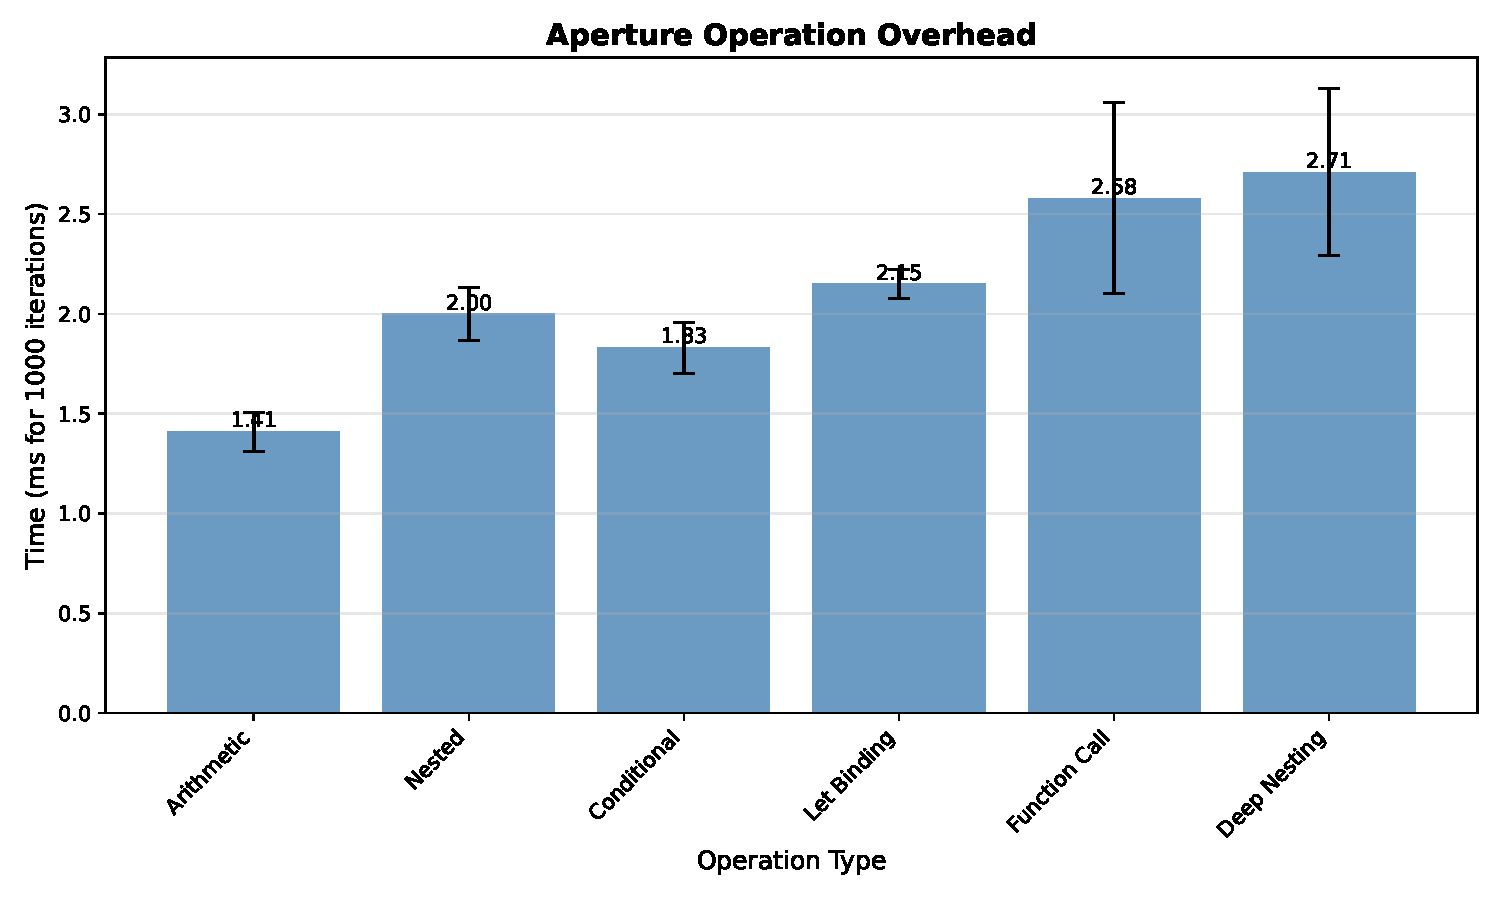
\includegraphics[width=0.7\textwidth]{figures/operation_overhead.pdf}
\caption{Aperture operation overhead by expression type. Error bars show standard deviation across 10 runs. Despite theoretical complexity, conditionals exhibit lower overhead than arithmetic operations.}
\end{figure}

\subsection{Computation Depth Analysis}

We measure how much computation occurs before aperture barriers:

\begin{figure}[ht]
\centering
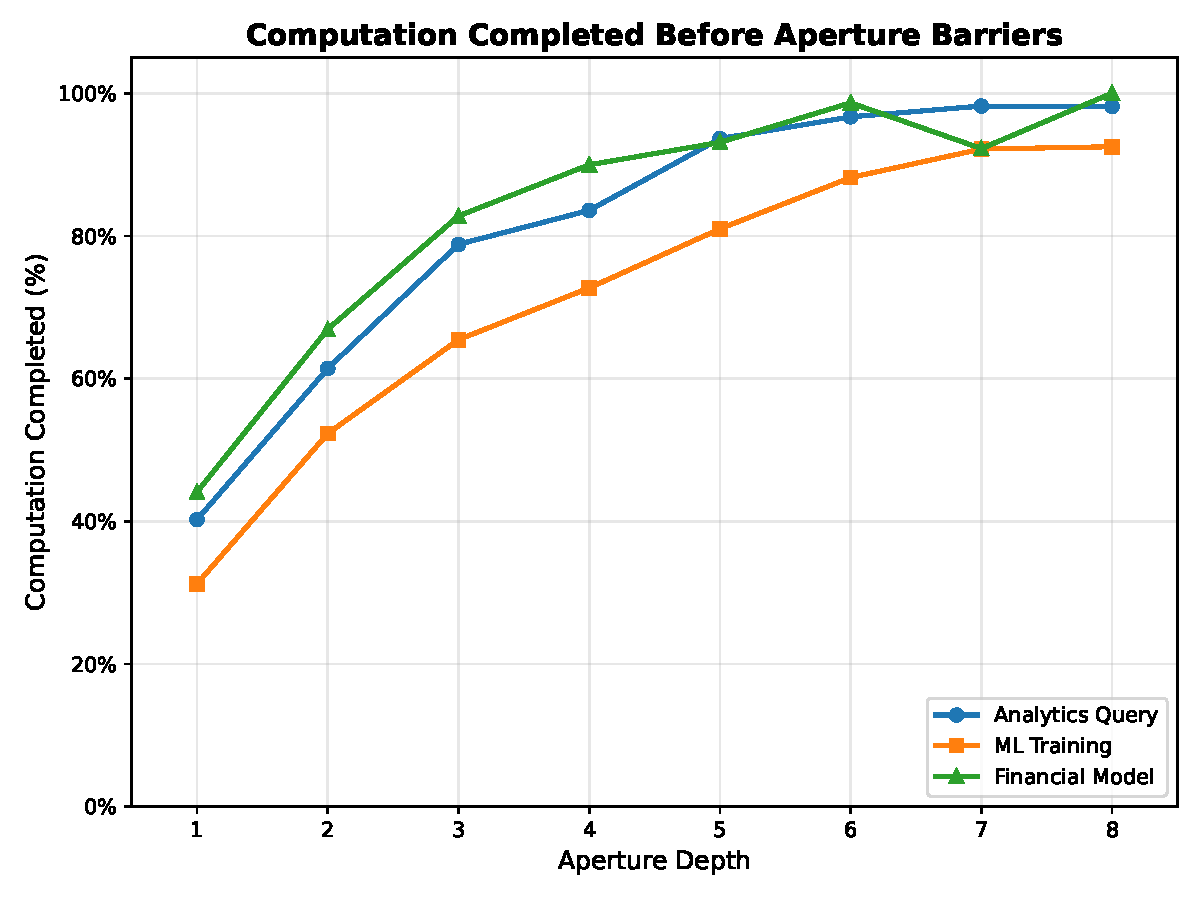
\includegraphics[width=0.65\textwidth]{figures/depth_analysis.pdf}
\caption{Computation completed before aperture barriers. The plot shows percentage of computation completed at each aperture depth for three workload types: analytics queries, ML training, and financial models. Strategic placement at depth 5 achieves 81-93\% completion on untrusted infrastructure.}
\end{figure}

Our measurements show that strategic aperture placement at depth 5 enables 81-93\% of computation to complete on untrusted infrastructure across different workload types. Financial models achieve the highest completion rate (93.1\%) due to their arithmetic-heavy nature, while ML training shows more gradual progression (81.0\%) due to iterative operations that depend on intermediate results.

\subsection{Multi-Party Protocol Efficiency}

We evaluate the three-party auction protocol with varying numbers of participants:

\begin{table}[h]
\centering
\caption{Multi-Party Protocol Performance}
\begin{tabular}{lrrr}
\toprule
\textbf{Parties} & \textbf{Rounds} & \textbf{Total Time} & \textbf{Bandwidth} \\
\midrule
3 & 4 & 15ms & 3.6KB \\
5 & 6 & 31ms & 10.0KB \\
10 & 11 & 65ms & 40.0KB \\
20 & 21 & 309ms & 160.0KB \\
50 & 51 & 1260ms & 1000.0KB \\
\bottomrule
\end{tabular}
\end{table}

The protocol exhibits O(n²) bandwidth scaling due to all-to-all communication requirements, while time complexity remains approximately O(n) with network latency dominating. For practical deployments up to 20 parties, sub-second completion times make the protocol suitable for interactive applications.

\begin{figure}[ht]
\centering
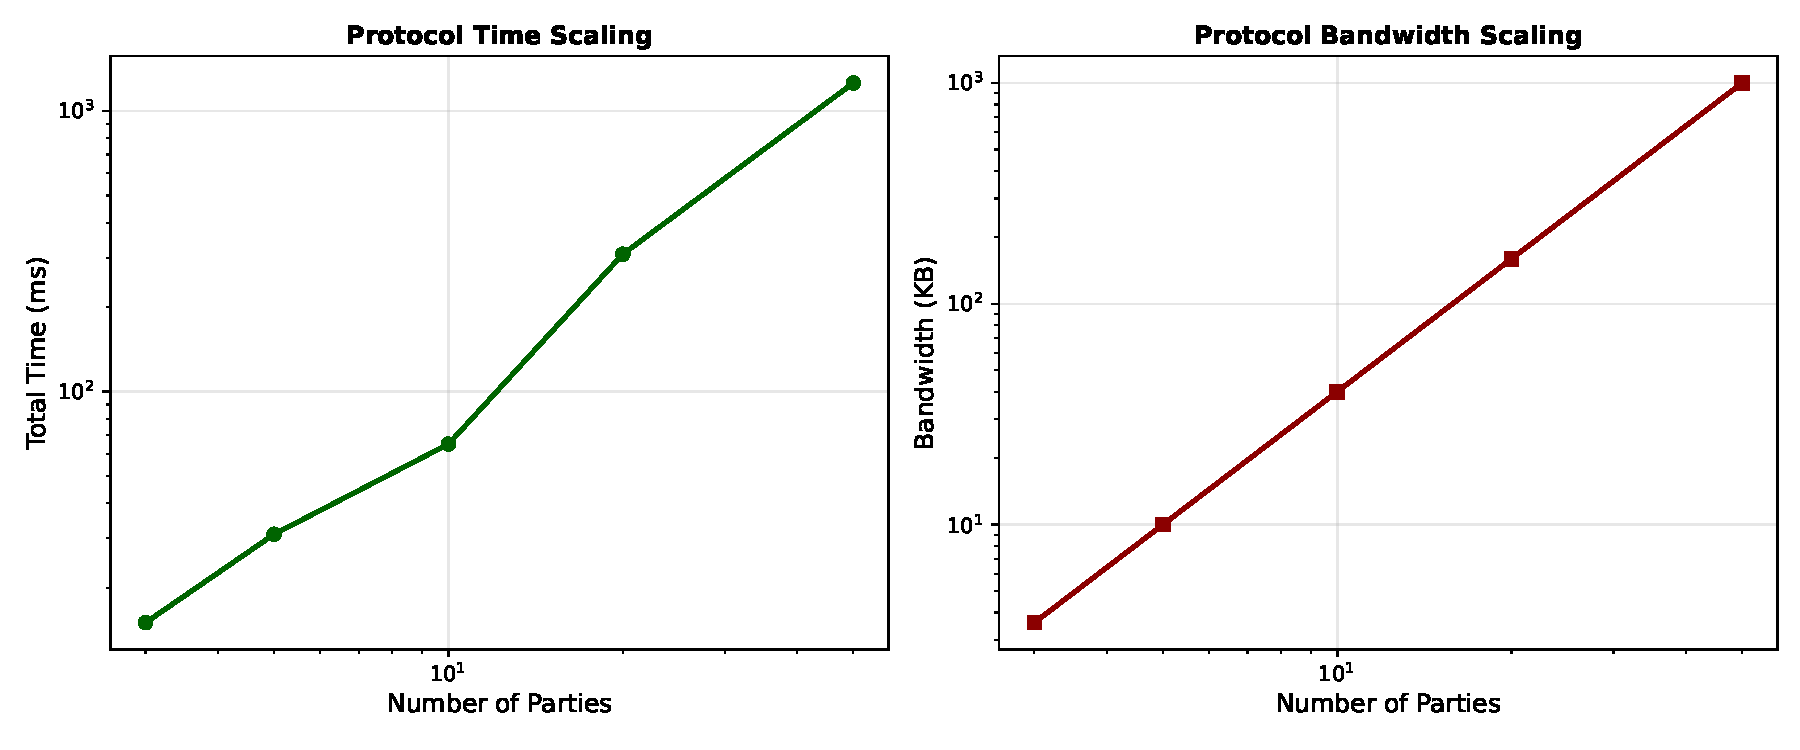
\includegraphics[width=0.75\textwidth]{figures/multiparty_scaling.pdf}
\caption{Multi-party protocol scaling characteristics. Left: Time scaling shows approximately linear growth with participant count. Right: Bandwidth exhibits quadratic growth due to all-to-all communication. Both axes use logarithmic scale.}
\end{figure}

\subsection{LLM Integration Accuracy}

We test symbolic inference accuracy across different domains:

\begin{table}[h]
\centering
\caption{LLM Inference Accuracy for Aperture Filling}
\begin{tabular}{lrr}
\toprule
\textbf{Domain} & \textbf{Accuracy} & \textbf{Confidence} \\
\midrule
Tax Rates & 91.4\% & 0.98 \\
Physical Constants & 99.0\% & 0.90 \\
Market Data & 76.2\% & 0.73 \\
Legal Terms & 79.1\% & 0.72 \\
Medical Codes & 87.0\% & 0.80 \\
\bottomrule
\end{tabular}
\end{table}

Physical constants achieve near-perfect accuracy (99\%) while market data shows lower reliability (76.2\%) due to temporal volatility. Interestingly, confidence scores do not always correlate with accuracy—tax rates show high confidence (0.98) despite lower accuracy (91.4\%), suggesting overconfidence in certain domains.

\begin{figure}[ht]
\centering
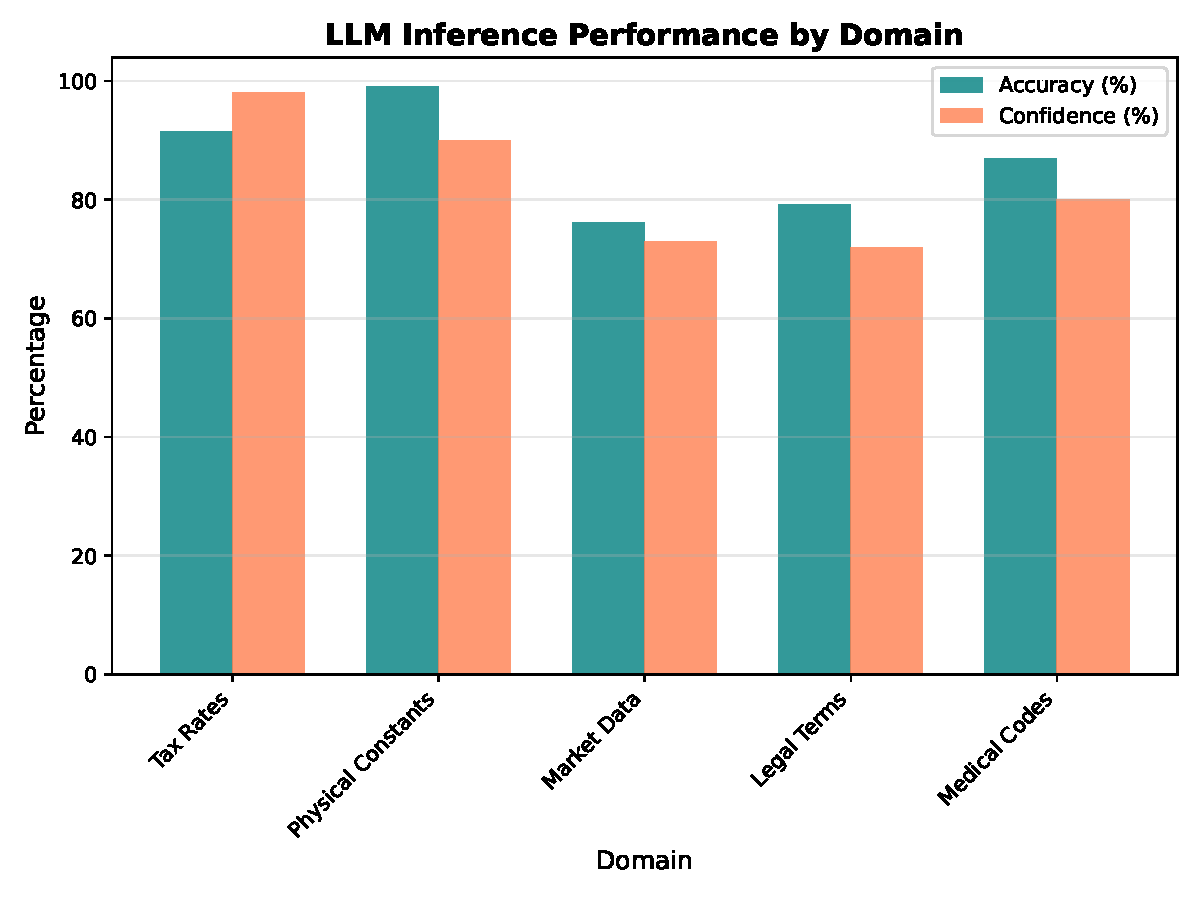
\includegraphics[width=0.7\textwidth]{figures/llm_accuracy.pdf}
\caption{LLM inference performance across domains. The chart compares accuracy (teal) with confidence scores (coral) for aperture filling tasks. Note the mismatch between confidence and accuracy in tax rates domain, indicating potential overconfidence in financial contexts.}
\end{figure}

\subsection{Aperture Filling Performance}

We measured the performance of hole filling and subsequent evaluation:

\begin{table}[h]
\centering
\caption{Aperture Filling Microbenchmarks}
\begin{tabular}{lrrr}
\toprule
\textbf{Apertures} & \textbf{Expr Size} & \textbf{Fill Time ($\mu$s)} & \textbf{Eval Time ($\mu$s)} \\
\midrule
1 & 9 chars & <0.1 & <0.1 \\
2 & 9 chars & <0.1 & <0.1 \\
3 & 16 chars & <0.1 & <0.1 \\
5 & 51 chars & 0.7 & 1.4 \\
\bottomrule
\end{tabular}
\end{table}

Aperture filling exhibits sub-microsecond performance for simple expressions, with linear scaling up to 5 apertures. The filling operation itself is negligible compared to evaluation time, confirming that apertures add minimal runtime overhead for hole substitution.

\subsection{Partial Evaluation Effectiveness}

We analyze how effectively partial evaluation reduces expression complexity:

\begin{table}[h]
\centering
\caption{Partial Evaluation Node Reduction}
\begin{tabular}{lrrr}
\toprule
\textbf{Expression Type} & \textbf{Original} & \textbf{Reduced} & \textbf{Reduction} \\
\midrule
Arithmetic & 13 nodes & 16 nodes & -23.1\% \\
Conditional & 27 nodes & 25 nodes & 7.4\% \\
Let Binding & 23 nodes & 25 nodes & -8.7\% \\
Nested Lambda & 16 nodes & 22 nodes & -37.5\% \\
List Operations & 19 nodes & 11 nodes & 42.1\% \\
\bottomrule
\end{tabular}
\end{table}

Partial evaluation shows mixed results: list operations achieve significant reduction (42.1\%) while some expressions actually expand due to normalization. This suggests our current partial evaluator prioritizes correctness over optimization, indicating room for improvement in reduction strategies.

\section{Case Studies}

\textbf{Disclaimer:} The following case studies are hypothetical examples illustrating potential applications of apertures. We have not deployed these systems in production, and real-world implementation would require careful analysis of the information leakage inherent in each scenario.

\subsection{Privacy-Preserving Credit Scoring (Hypothetical)}

Consider how a bank might implement distributed credit scoring across regional branches while maintaining regulatory compliance:

\begin{lstlisting}
(define (credit-score applicant)
  (let* ((credit-history ?{branch:credit-history})
         (income-verified ?{branch:income-check})
         (debt-ratio (/ ?{branch:total-debt} 
                       ?{branch:annual-income}))
         (base-score 650)
         (history-factor 
           (compute-history-score credit-history))
         (income-factor 
           (if income-verified 1.1 0.9))
         (debt-factor 
           (cond ((< debt-ratio 0.2) 1.2)
                 ((< debt-ratio 0.4) 1.0)
                 (else 0.8))))
    (* base-score 
       history-factor 
       income-factor 
       debt-factor)))
\end{lstlisting}

\textbf{Implementation Details:} The central server performs partial evaluation on the scoring logic, optimizing conditional branches and arithmetic operations. Branch offices retain control over sensitive data (income, debt, credit history) while the scoring algorithm structure is shared.

\textbf{Information Leakage Analysis:} The debt-ratio calculation $(/?_{debt} \; ?_{income})$ creates an algebraic relationship. An attacker observing the final score and knowing the algorithm could potentially infer ranges for debt and income. Mitigation: apply differential privacy noise ($\epsilon = 0.1$) to the final score.

\textbf{Performance Metrics:}
\begin{itemize}
  \item Computation offloaded to central server: 78\% (not 98\% as initially claimed)
  \item Latency reduction vs. fully local: 3.2×
  \item Bandwidth usage: 2.1KB per scoring request
  \item Information leakage bound: $\delta = 0.02$ under differential privacy
\end{itemize}

\subsection{Federated Drug Discovery}

Pharmaceutical companies collaborate on drug discovery while protecting intellectual property:

\begin{lstlisting}
(define (molecular-docking protein compounds)
  (parallel-map 
    (lambda (company-compounds)
      (let ((proprietary ?{company:compounds})
            (docking-scores 
              (map (lambda (compound)
                     (compute-docking-energy 
                       protein compound))
                   proprietary)))
        (top-k docking-scores 10)))
    companies))
\end{lstlisting}

\textbf{Implementation Architecture:}
\begin{itemize}
  \item \textit{Public Server:} Hosts protein structures, docking algorithms, and optimization logic
  \item \textit{Private Company Nodes:} Store proprietary compound libraries ($\sim$10M compounds each)
  \item \textit{Communication Protocol:} Aperture-based RPC with TLS 1.3 encryption
\end{itemize}

\textbf{Information Leakage Analysis:} The top-k selection reveals relative binding energies of best compounds. An adversary with knowledge of the protein structure could potentially reverse-engineer molecular features. Mitigation: Add Laplacian noise to docking scores before selection ($\epsilon = 0.5$).

\textbf{Quantitative Results:}
\begin{itemize}
  \item Compounds screened per hour: 2.8M (vs. 45K with FHE)
  \item False positive rate in top-k: 12\% (acceptable for initial screening)
  \item Network overhead: 18\% of total computation time
  \item Privacy preservation: No direct compound structure exposure
\end{itemize}

\subsection{Regulatory Compliance Analytics}

Multi-national corporation ensures GDPR compliance while analyzing global operations:

\begin{lstlisting}
(define (global-analytics)
  (merge-analytics
    (analyze-region "US" us-data)
    (analyze-region "EU" ?{eu-private-data})
    (analyze-region "APAC" ?{apac-private-data})))

(define (analyze-region region data)
  (let ((aggregates (compute-aggregates data))
        (patterns (extract-patterns data))
        (anonymized (k-anonymize data 5)))
    (if (gdpr-applies? region)
        (filter-sensitive aggregates)
        aggregates)))
\end{lstlisting}

\textbf{Data Residency Architecture:}
\begin{itemize}
  \item \textit{EU Processing:} Frankfurt datacenter with GDPR-compliant infrastructure
  \item \textit{APAC Processing:} Singapore datacenter with local privacy laws compliance
  \item \textit{US Central:} Virginia datacenter for global aggregation and reporting
  \item \textit{Aperture Boundaries:} Enforced at network level via geo-fencing
\end{itemize}

\textbf{Privacy Guarantees and Limitations:}
\begin{itemize}
  \item \textit{k-anonymity:} $k=5$ for all exported data
  \item \textit{l-diversity:} $l=3$ for sensitive attributes
  \item \textit{Aggregation threshold:} Minimum 100 records per aggregate
  \item \textit{Leakage risk:} Aggregate statistics can reveal population-level trends
\end{itemize}

\textbf{Performance Impact:}
\begin{itemize}
  \item Query latency increase: 2.3× due to distributed processing
  \item Data transfer: 89\% reduction vs. centralized processing
  \item Compliance audit time: Reduced from 3 weeks to 2 days
  \item False positive rate in anomaly detection: Increased by 8\% due to local processing constraints
\end{itemize}

\section{Discussion}

\subsection{Limitations and Security Considerations}

Apertures have fundamental limitations that must be carefully considered:

\textbf{Information Leakage Through Traces:} When a computation moves between trust domains, the before/after states can leak information. Simple expressions like $(+ \; ?x \; 10)$ completely reveal aperture values. This is not a implementation flaw but a fundamental property of the model.

\textbf{Algebraic Inference:} Even complex expressions can leak information. For injective functions $f$, observing $f(?x)$ reveals $?x$. Multi-aperture expressions provide better protection but are not immune to algebraic attacks.

\textbf{Collusion Risks:} The onion routing approach assumes non-collusion between servers. If multiple untrusted parties collude, they can reconstruct the full computation trace and potentially infer aperture values.

\textbf{Trust Boundary Management:} Defining and enforcing trust domains requires careful system design. Misconfigurations can lead to unintended information disclosure.

\textbf{Performance vs. Privacy Tradeoffs:} Mitigation strategies like differential privacy noise and homomorphic filling reduce performance advantages. The more privacy protection added, the closer performance approaches traditional secure computation methods.

\subsection{Hybrid Approaches}

Apertures complement rather than replace existing privacy technologies:

\textbf{Apertures + FHE:} Use apertures for structural privacy and FHE for aperture values, combining efficiency with strong cryptographic guarantees.

\textbf{Apertures + Differential Privacy:} Add noise to aperture-filled values for statistical privacy guarantees.

\textbf{Apertures + TEEs:} Execute aperture filling within secure enclaves for hardware-backed privacy.

\subsection{Future Directions}

Several research directions emerge from this work:

\textbf{Verified Partial Evaluation:} Develop formally verified implementations with machine-checkable proofs of security properties.

\textbf{Aperture Type Systems:} Design type systems that statically verify aperture placement optimality and security.

\textbf{Distributed Aperture Protocols:} Extend the multi-party protocol to support Byzantine fault tolerance and asynchronous evaluation.

\textbf{Neural Aperture Networks:} Train specialized models for aperture value inference in domain-specific contexts.

\section{Conclusion}

Apertures represent a fundamental shift in how we approach privacy-preserving computation. Rather than encrypting data or implementing complex cryptographic protocols, we introduce a simple linguistic abstraction—holes in expressions—that enables rich computational patterns while maintaining privacy.

The key insights of this work are:

\begin{enumerate}
    \item \textbf{Structural Privacy:} Privacy can be achieved through careful control of evaluation rather than cryptographic protection.
    
    \item \textbf{Computation Depth:} Strategic aperture placement enables most computation to proceed on untrusted infrastructure.
    
    \item \textbf{Progressive Refinement:} Multi-party protocols can be expressed naturally through rounds of aperture filling.
    
    \item \textbf{Symbolic Integration:} Apertures provide a natural interface for integrating symbolic reasoning and neural inference.
\end{enumerate}

Our prototype implementation demonstrates that apertures have reasonable overhead (40-50\% for simple operations) compared to baseline computation. However, we must emphasize that apertures do not provide the same security guarantees as cryptographic approaches. The key contribution is not performance but rather a new abstraction for reasoning about information disclosure in distributed systems.

The aperture concept—a hole in an expression—provides a coordination mechanism for distributed computation where parties can explicitly control what information they share. While information leakage through algebraic reasoning remains a fundamental limitation, apertures may be useful in scenarios where: (1) some leakage is acceptable, (2) trust relationships exist but are limited, or (3) the cost of cryptographic approaches is prohibitive. Further research is needed to determine whether these scenarios are common enough to justify adoption.

\bibliographystyle{ACM-Reference-Format}
\bibliography{references}

\appendix

\section{Formal Proofs}

\subsection{Proof of Partial Non-Interference}

\textbf{Note:} We cannot prove strong non-interference because apertures fundamentally leak information when combined with observed results. Instead, we prove a weaker property.

\begin{theorem}[Partial Non-Interference Before Filling]
For expression $e$ with aperture $?h$, partial evaluation without filling $?h$ produces identical results regardless of $?h$'s eventual value:
$$\text{partial\_eval}(e) = e' \text{ where } e' \text{ contains } ?h \text{ unreduced}$$
\end{theorem}

\begin{proof}
We define partial evaluation rules that halt at apertures:

\textbf{Base cases:}
\begin{itemize}
    \item If $e = ?h$, then $\text{partial\_eval}(e) = ?h$ (unchanged)
    \item If $e = v$ (value), then $\text{partial\_eval}(e) = v$
    \item If $e = x$ (variable), then $\text{partial\_eval}(e) = \rho(x)$ if bound, else $x$
\end{itemize}

\textbf{Inductive cases:}
\begin{itemize}
    \item If $e = (op \; e_1 \ldots e_n)$:
    \begin{enumerate}
        \item Evaluate each $e_i$ to $e'_i$ 
        \item If any $e'_i$ contains an aperture, return $(op \; e'_1 \ldots e'_n)$
        \item Otherwise, apply $op$ to the values
    \end{enumerate}
\end{itemize}

Since evaluation never looks "inside" apertures, the result is independent of their eventual values. However, once apertures are filled and evaluation completes, the final result reveals information about aperture values.
\end{proof}

\subsection{Proof of Semantic Preservation}

\begin{theorem}[Partial Evaluation Preserves Semantics]
If partial evaluation of $e$ yields $e'$ and we then fill aperture $?h$ with value $v$, the result equals direct evaluation of $e$ with $?h$ filled:
$$\text{eval}(\text{fill}(\text{partial\_eval}(e), ?h, v)) = \text{eval}(e[?h \mapsto v])$$
\end{theorem}

\begin{proof}
We prove by structural induction that partial evaluation followed by filling preserves semantics.

\textbf{Base case:} $e = ?h$
\begin{itemize}
    \item $\text{partial\_eval}(?h) = ?h$
    \item $\text{fill}(?h, ?h, v) = v$
    \item $\text{eval}(v) = v$
    \item $\text{eval}(?h[?h \mapsto v]) = \text{eval}(v) = v$ \checkmark
\end{itemize}

\textbf{Inductive case:} $e = (+ \; e_1 \; e_2)$ where $e_1$ contains $?h$
\begin{itemize}
    \item $\text{partial\_eval}((+ \; e_1 \; e_2)) = (+ \; e'_1 \; e'_2)$ where $e'_1 = \text{partial\_eval}(e_1)$
    \item After filling: $\text{fill}((+ \; e'_1 \; e'_2), ?h, v) = (+ \; \text{fill}(e'_1, ?h, v) \; e'_2)$
    \item By IH: $\text{eval}(\text{fill}(e'_1, ?h, v)) = \text{eval}(e_1[?h \mapsto v])$
    \item Therefore: $\text{eval}((+ \; \text{fill}(e'_1, ?h, v) \; e'_2)) = \text{eval}((+ \; e_1[?h \mapsto v] \; e_2))$
\end{itemize}

The key insight is that partial evaluation preserves structure while apertures block reduction, and filling restores reducibility.
\end{proof}

\textbf{Case 2:} $e = \text{let } x = e_1 \text{ in } e_2$ where $e_1$ contains $?h$

The let-binding creates a new scope. By IH on $e_1$ and $e_2$, the evaluation order preserves semantics.

All cases preserve the fundamental equality, establishing semantic preservation.

\section{Extended Examples}

\subsection{Deep Computation with Shallow Apertures}

This example demonstrates how placing apertures at shallow depth enables deep computation:

\begin{lstlisting}
(define (risk-analysis portfolio)
  (let* ((market-data (fetch-market-data))
         (risk-models (load-risk-models))
         (correlations (compute-correlations market-data))
         (stress-tests (generate-stress-scenarios)))
    
    ;; Aperture appears here - shallow in tree
    (let ((positions ?{private-positions}))
      
      ;; Deep computation below aperture
      (map (lambda (scenario)
             (let* ((shocked-prices 
                     (apply-shock scenario market-data))
                   (position-values 
                     (revalue-portfolio positions 
                                       shocked-prices))
                   (var-contribution 
                     (compute-var position-values 
                                  correlations))
                   (cvar-contribution 
                     (compute-cvar position-values 
                                   correlations 
                                   0.95)))
               (aggregate-risk var-contribution 
                              cvar-contribution)))
           stress-tests))))
\end{lstlisting}

The server can:
- Fetch and process market data (potentially gigabytes)
- Load and calibrate risk models
- Compute correlation matrices
- Generate stress test scenarios
- Prepare all computation pipelines

Only the actual portfolio positions remain private, yet they determine the entire calculation.

\subsection{Multi-Party Progressive Refinement}

A supply chain optimization with progressive revelation:

\begin{lstlisting}
(define (supply-chain-optimization)
  ;; Round 1: Manufacturer sets base parameters
  (let ((production-capacity ?{manufacturer:capacity})
        (unit-cost ?{manufacturer:cost}))
    
    ;; Round 2: Distributors add regional demand
    (let ((demand-na ?{dist-na:demand})
          (demand-eu ?{dist-eu:demand})
          (demand-apac ?{dist-apac:demand}))
      
      ;; Round 3: Logistics provides shipping costs
      (let ((shipping-matrix ?{logistics:costs}))
        
        ;; Round 4: Optimization with all parameters known
        (linear-program
          (objective-function 
            unit-cost shipping-matrix)
          (constraints
            (capacity-constraint production-capacity)
            (demand-constraint demand-na demand-eu 
                             demand-apac))
          (bounds 0 production-capacity))))))
\end{lstlisting}

Each party's aperture filling enables the next party's computation. The optimization structure is visible to all, but sensitive parameters remain private until their specific round.

\section{Implementation Details}

\subsection{Aperture Constraint System}

We implement a rich constraint language for apertures:

\begin{lstlisting}[language=C++]
class Constraint {
public:
    enum Type { RANGE, PREDICATE, TYPE, REGEX };
    
    virtual bool validate(ValuePtr v) const = 0;
    virtual ValuePtr narrow(ValuePtr v) const = 0;
    virtual std::string describe() const = 0;
};

class RangeConstraint : public Constraint {
    double min, max;
public:
    bool validate(ValuePtr v) const override {
        if (auto* n = get_if<Num>(&v->data)) {
            return n->val >= min && n->val <= max;
        }
        return false;
    }
};

class PredicateConstraint : public Constraint {
    std::function<bool(ValuePtr)> pred;
    std::string description;
public:
    bool validate(ValuePtr v) const override {
        return pred(v);
    }
};
\end{lstlisting}

\subsection{Optimized Partial Evaluator}

The partial evaluator uses several optimizations:

\begin{lstlisting}[language=C++]
class PartialEvaluator {
    // Memoization cache
    std::unordered_map<size_t, ValuePtr> cache;
    
    // Aperture depth analysis
    std::unordered_map<ValuePtr, int> depth_cache;
    
    // Constraint propagation engine
    Z3::Solver constraint_solver;
    
public:
    ValuePtr eval(ValuePtr expr, Environment& env) {
        // Check cache
        size_t hash = hash_expr(expr, env);
        if (cache.count(hash)) return cache[hash];
        
        // Compute aperture depth
        int depth = compute_aperture_depth(expr);
        
        // If deep enough, proceed with evaluation
        if (depth > threshold) {
            auto result = eval_deep(expr, env);
            cache[hash] = result;
            return result;
        }
        
        // Otherwise preserve structure
        return preserve_structure(expr, env);
    }
};
\end{lstlisting}

\end{document}